\chapter{Filesystem Performance}

Performance is a fascinating but complex subject with a lot of "depends on" as part of the conversation. Since file activity is such a critical part of making a system \textit{perform} there have been many changes to the kernel over several decades to get the best performance possible. In addition to the kernel, filesystems and underlying storage subsystems have made huge advances

Whole books have been written about operating system performance. This chapter can only go so far but will explain areas of the kernel that affect performance, cover performance studies of different filesystems and describes the tools available that can help analyze performance bottlenecks.

Brendan Gregg's book \textit{Systems Performance -- Enterprise and the Cloud} \cite{gregg-perf} is \textbf{XXX}

% https://access.redhat.com/documentation/en-us/red_hat_enterprise_linux/8/html/monitoring_and_managing_system_status_and_performance/factors-affecting-i-o-and-file-system-performance_monitoring-and-managing-system-status-and-performance - factors affecting FS performance

\section{Performance of Different Filesystems}

Linux supports over 80 different filesystem types although less than 10 of them could be considered high-performance filesystems. Which one to use is going to depend both on the type of I/O that the application is performing as well as the underlying storage subsystem.

This section describes the performance characteristics of the major filesystems referencing various studies that have taken place over recent years.

\subsection{The Phoronix Study}

The Phoronix study in 2019 tested the performance of btrfs, ext4, XFS and F2FS on aSATA 3.0 solid-state drive, USB SSD, and an NVMe SSD.

The conclusion of the tests were that F2FS and XFS are usually fastest on the consumer solid-state storage devices with ext4 not too far behind. Btrfs has a lot of features but at least in its out-of-the-box behavior generally being a fair amount slower than EXT4/F2FS/XFS. Perhaps most interesting from today's results were the startup-time application results where the Flash-Friendly File-System easily won across all of those tests. \textbf{XXX---needs to be rewritten - copied from page 4}

You can find the study here:

\begin{table}[h]
\begin{tabular}{lcl}
\parbox[r]{0.5in}{
\includegraphics[scale=0.15]{figures/url.png}} & \parbox[l]{0.5in}{URL \arabic{urls} -- } & \parbox[l]{3in}{\cf{https://tinyurl.com/4yu4zef8}}
\end{tabular}
\end{table}
\stepcounter{urls}
% https://www.phoronix.com/review/linux-50-filesystems

%https://www.linux-magazine.com/Online/Features/Filesystems-Benchmarked

\section{Mount Options}

TBD

%https://www.linux-magazine.com/Online/Features/Filesystems-Benchmarked etc

\section{Block Sizes}

TBD

%

\section{Extend-based Allocation}

TBD

\section{The Effects of Filesystem Fragmentation}

TBD

%https://cromwell-intl.com/open-source/performance-tuning/file-systems.html

\section{Open Flags etc etc}

TBD - depends on which FS

%

\section{Volume Management / Disk Subsystems}

things have changed a lot - cloud???

SSDs vs ...

%

\section{Buffer Cache and Page Cache Tuning}

free command to show buf/cache usage

%https://www.baeldung.com/linux/empty-buffer-cache

\section{Other commands???}

\section{The \cf{sysstat} Package}

The \cf{sysstat} package contains various utilities, common to many commercial Unixes, to monitor system performance and usage activity:

\begin{table}[h]
\begin{tabular}{lcl}
\parbox[r]{0.5in}{
\includegraphics[scale=0.15]{figures/url.png}} & \parbox[l]{0.5in}{URL \arabic{urls} -- } & \parbox[l]{3in}{\cf{https://tinyurl.com/5auz66fj}}
\end{tabular}
\end{table}
\stepcounter{urls}
% https://github.com/sysstat/sysstat

\noindent
Here are the standalone commands that are part of the package. I'm the description text from the website

\begin{itemize}
	\item \cf{iostat} -- reports CPU statistics and input/output statistics for block devices and partitions.
	\item \cf{mpstat} -- reports individual or combined processor related statistics.
	\item \cf{pidstat} -- reports statistics for Linux tasks (processes) : I/O, CPU, memory, etc.
	\item \cf{tapestat} -- reports statistics for tape drives connected to the system.
	\item \cf{cifsiostat} -- reports CIFS statistics.
\end{itemize}

\noindent
There are also tools in the package that can be scheduled via \cf{cron} or \cf{systemd} to collect and historize performance and activity data:

\begin{itemize}
	\item \cf{sar} -- collects, reports and saves system activity information (see below a list of metrics collected by sar).
	\item \cf{sadc} -- is the system activity data collector, used as a backend for sar.
	\item \cf{sa1} -- collects and stores binary data in the system activity daily data file. It is a front end to sadc 
		designed to be run from cron or systemd.
	\item \cf{sa2} -- writes a summarized daily activity report. It is a front end to sar designed to be run from cron or systemd.
	\item \cf{sadf} -- displays data collected by sar in multiple formats (CSV, XML, JSON, etc.) and can be used f
		or data exchange with other programs. This command can also be used to draw graphs for the various 
		activities collected by sar using SVG (Scalable Vector Graphics) format.
\end{itemize}

\noindent
The default sampling interval for these tools is 10 minutes but this value can be changed and be as low as 1 second.

After installing the package, if you try to run one of these tools you may see:

\begin{lstlisting}
$ [*\bfseries sudo sar*]
[sudo] password for spate: 
Cannot open /var/log/sysstat/sa26: No such file or directory
Please check if data collecting is enabled
\end{lstlisting}

\noindent
To enable collection of data you need to edit the file \cf{/etc/default/sysstat} and change \cf{ENABLED="false"} to \cf{ENABLED="true"} and then run:

\begin{lstlisting}
$ [*\bfseries sudo service sysstat restart
\end{lstlisting}

\section{eBPF -- a New World of Opportunities}

The \textit{Berkeley Packet Filter (BPF)} is a technology that originated in BSD UNIX in 1992 for programs that need to, among other things, analyze network traffic. It provided a raw interface to data link layers in a protocol independent fashion. All packets on the network, even those destined for other hosts, are accessible through this mechanism.

eBPF, the \textit{extended Berkeley Packet Filter}, is a technology. It has a lot of promise as performance expert Brendan Gregg has been quoted as saying.

\begin{quote}
\textit{"super powers have finally come to Linux"} -- Brendan Gregg
\end{quote}

\noindent
Gregg's book \textit{BPF Performance Tools} \cite{gregg-ebpf} provides in-depth information about eBPF covering everything from XXX to YYY. There is also a significant amount of information in his website:

eBPF is a technology that allows programs to be run in the kernel in a sandboxed environment. It does this XXX

best description here - https://ebpf.io/what-is-ebpf/

\begin{table}[h]
\begin{tabular}{lcl}
\parbox[r]{0.5in}{
\includegraphics[scale=0.15]{figures/url.png}} & \parbox[l]{0.55in}{URL \arabic{urls} -- } & \parbox[l]{3in}{\cf{https://tinyurl.com/4hvpc35j}}
\end{tabular}
\end{table}
\stepcounter{urls}
% https://github.com/iovisor/bpftrace

\begin{table}[h]
\begin{tabular}{lcl}
\parbox[r]{0.5in}{
\includegraphics[scale=0.15]{figures/url.png}} & \parbox[l]{0.55in}{URL \arabic{urls} -- } & \parbox[l]{3in}{\cf{https://tinyurl.com/yc2y7kvy}}
\end{tabular}
\end{table}
\stepcounter{urls}
% https://www.brendangregg.com/ebpf.html

\noindent
Some aspects of eBPF have already been covered including how it can be used to enhance FUSE filesystem performance (section \ref{debug-ebpf}) and debugging to understand whether specific Linux kernel functions are invoked or not (section \ref{fuse-ebpf}).

Figure \ref{fig:ebpf} shows how it all works XXX

\begin{figure}
	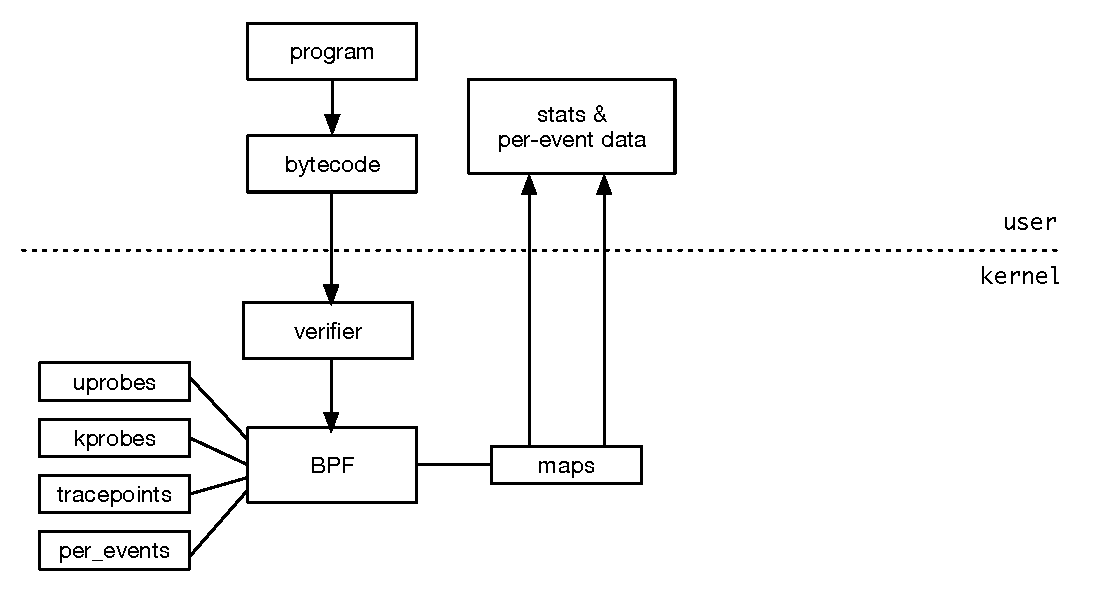
\includegraphics[scale=0.6]{figures/eBPF.pdf}
	\centering
	\caption{eBPF Flow - XXX}
	\label{fig:ebpf}
\end{figure}

\subsection{BCC -- BPF Compiler Collection}

TBD

The source code and information about BCC can be found on github here:

\begin{table}[h]
\begin{tabular}{lcl}
\parbox[r]{0.5in}{
\includegraphics[scale=0.15]{figures/url.png}} & \parbox[l]{0.55in}{URL \arabic{urls} -- } & \parbox[l]{3in}{\cf{https://tinyurl.com/fmfe8498}}
\end{tabular}
\end{table}
\stepcounter{urls}
% https://github.com/iovisor/bcc

\noindent
There are many examples shown at the bottom of the home page including tracing a kernel functions and printing all kernel stack traces and VFS read latency distribution (\textbf{XXX---explain or remove}.

\subsection{The \cf{bpftrace} Command}

BPFtrace is a high level tracing language which is built on top of LLVM and BCC. BPFtrace provides an easier way of writing BPF programs for interacting with Linux tracing capabilities, such as kprobes, uprobes, kernel tracepoints, USDT and hardware events.

\cf{bptrace} is part of the \cf{iovisor} project. Source code and informaiton can be found here:

\begin{table}[h]
\begin{tabular}{lcl}
\parbox[r]{0.5in}{
\includegraphics[scale=0.15]{figures/url.png}} & \parbox[l]{0.55in}{URL \arabic{urls} -- } & \parbox[l]{3in}{\cf{https://tinyurl.com/4hvpc35j}}
\end{tabular}
\end{table}
\stepcounter{urls}
% https://github.com/iovisor/bpftrace

\begin{lstlisting}
$ [*\bfseries sudo apt  install bpftrace*]
\end{lstlisting}

\noindent
A great example to show the power of eBPF is with the following example that uses kprobes to XXX

% https://github.com/iovisor/bpftrace/blob/master/docs/tutorial_one_liners.md - Lesson 12

\begin{lstlisting}
#include <linux/path.h>
#include <linux/dcache.h>

kprobe:vfs_open
{
    printf("Path: %s\n", 
           str(((struct path *)arg0)->dentry->d_name.name));
}
\end{lstlisting}

\noindent
The program is run as follows:

\begin{lstlisting}
$ [*\bfseries sudo bpftrace open-path.bt*]
Attaching 1 probe...
Path: cgroup
Path: cat
Path: ld-linux-aarch64.so.1
Path: ld.so.cache
Path: libc.so.6
Path: locale-archive
Path: open-path.bt
...
\end{lstlisting}

\noindent
There will be a lot of output even on what seems like a Linux system with little activity. The first and last entry shown corresponded to running:

\begin{lstlisting}
$ [*\bfseries cat /home/spate/open-path.bt *]
\end{lstlisting}

\noindent
So very powerful XXX

\subsection{The Annual eBPF summit}

Each year there is an eBPF summit which is free to attend and covers many aspects of eBPF including new innovations. The summit started in 2020 so at the time of writing, there have been three conferences to date. Their website can be found here:

\begin{table}[h]
\begin{tabular}{lcl}
\parbox[r]{0.5in}{
\includegraphics[scale=0.15]{figures/url.png}} & \parbox[l]{0.55in}{URL \arabic{urls} -- } & \parbox[l]{3in}{\cf{https://ebpf.io}}
\end{tabular}
\end{table}
\stepcounter{urls}
% https://ebpf.io

\noindent
You can watch all of the videos and download slides for many of them. Example talks from the 2022 summit are:

\begin{itemize}
	\item The future of eBPF in the Linux Kernel -- vision from Alexei Starovoitov who is the co-creator and co-maintainer 
		of eBPF.
	\item eBPF - The Capital Market's Perspective -- VCs are showing interest in companies developing 
		eBPF-based technology.
	\item XRP: In-Kernel Storage Functions with eBPF
\end{itemize}

\noindent
If you're interested in learning more about eBPF, these short videos can help you gain a good understanding of the technology and its applications.

\section{Conclusion}

TBD